\section{Decyzje projektowe}\label{sec:decyzje-projektowe}

Jedną z najważniejszych decyzji w trakcie realizacji projektu był wybór rodzaju kości, jaką miał odczytywać
i interpretować model sztucznej inteligencji.
Jako najistotniejsze kryterium wyznaczono liczbę ścian będącą potęgą liczby dwa
(już na wstępnym etapie projektowania odrzucając standardową kość sześciościenną)
w celu łatwej interpretacji wyniku w notacji binarnej, stosowanej powszechnie w informatyce, w tym w kryptografii.
W następnej kolejności szukano kompromisu pomiędzy łatwością w odczycie ścianek a generowaniem jak największej liczby
bitów jednym rzutem, czyli kości o jak największej liczbie ścianek.

Z dostępnych powszechnie na rynku kości tylko cztero-, ośmio- i szesnastościenne spełniają pierwszy z wymienionych wyżej kryteriów.
Kość czterościenną odrzucono ze względu na jej kształt ostrosłupa foremnego o podstawie trójkąta,
na której liczby zapisywane są na rogach, a nie ściankach (co pokazano na rys.~\ref{fig:k4}).
Kość czerościenną rozważono również w postaci niestandardowych kształtów kości, które pokazano na rys.~\ref{fig:nietypowe_modern_k4},
jednakże je również odrzucono z racji na bardzo niską dostępność na rynku. Kolejną przeszkodą była trudność
z interetacją pustych (zaokrąglonych) ścianek kości typu modern, pokazanej na rys.~\ref{fig:modern_k4},
lub problem z odczytem bardzo małych oznaczeń w przypadku ściętego ostrosłupa pokazanego na rys.~\ref{fig:nietypowe_k4}, 
które przestałyby być widoczne przy nawet niewielkim przechyleniu kości.

Kość szesnastościenną również odrzucono ze względu na mały rozmiar ścianek oraz stosunkowo niewielki kąt ich nachylenia względem siebie,
który sprawia, że na zdjęciu robionym idealnie nad kością widoczne jest kilka ścianek jednocześnie, jak pokazano na rys.~\ref{fig:k16}.
Z pozostałych opcji tylko na kości ośmiościennej (pokazanej na rys.~\ref{fig:k8}) widać z góry dokładnie jedną ściankę,
a do tego ma liczbę ścianek będącą potęgą liczby 2 (co jest atutem, ze względu na konieczność przetwarzania wyniku na system binarny), zatem to ten rodzaj kości został wybrany do użycia w projekcie.

\begin{figure}[h]
    \centering
      \begin{subfigure}{.3\textwidth}
        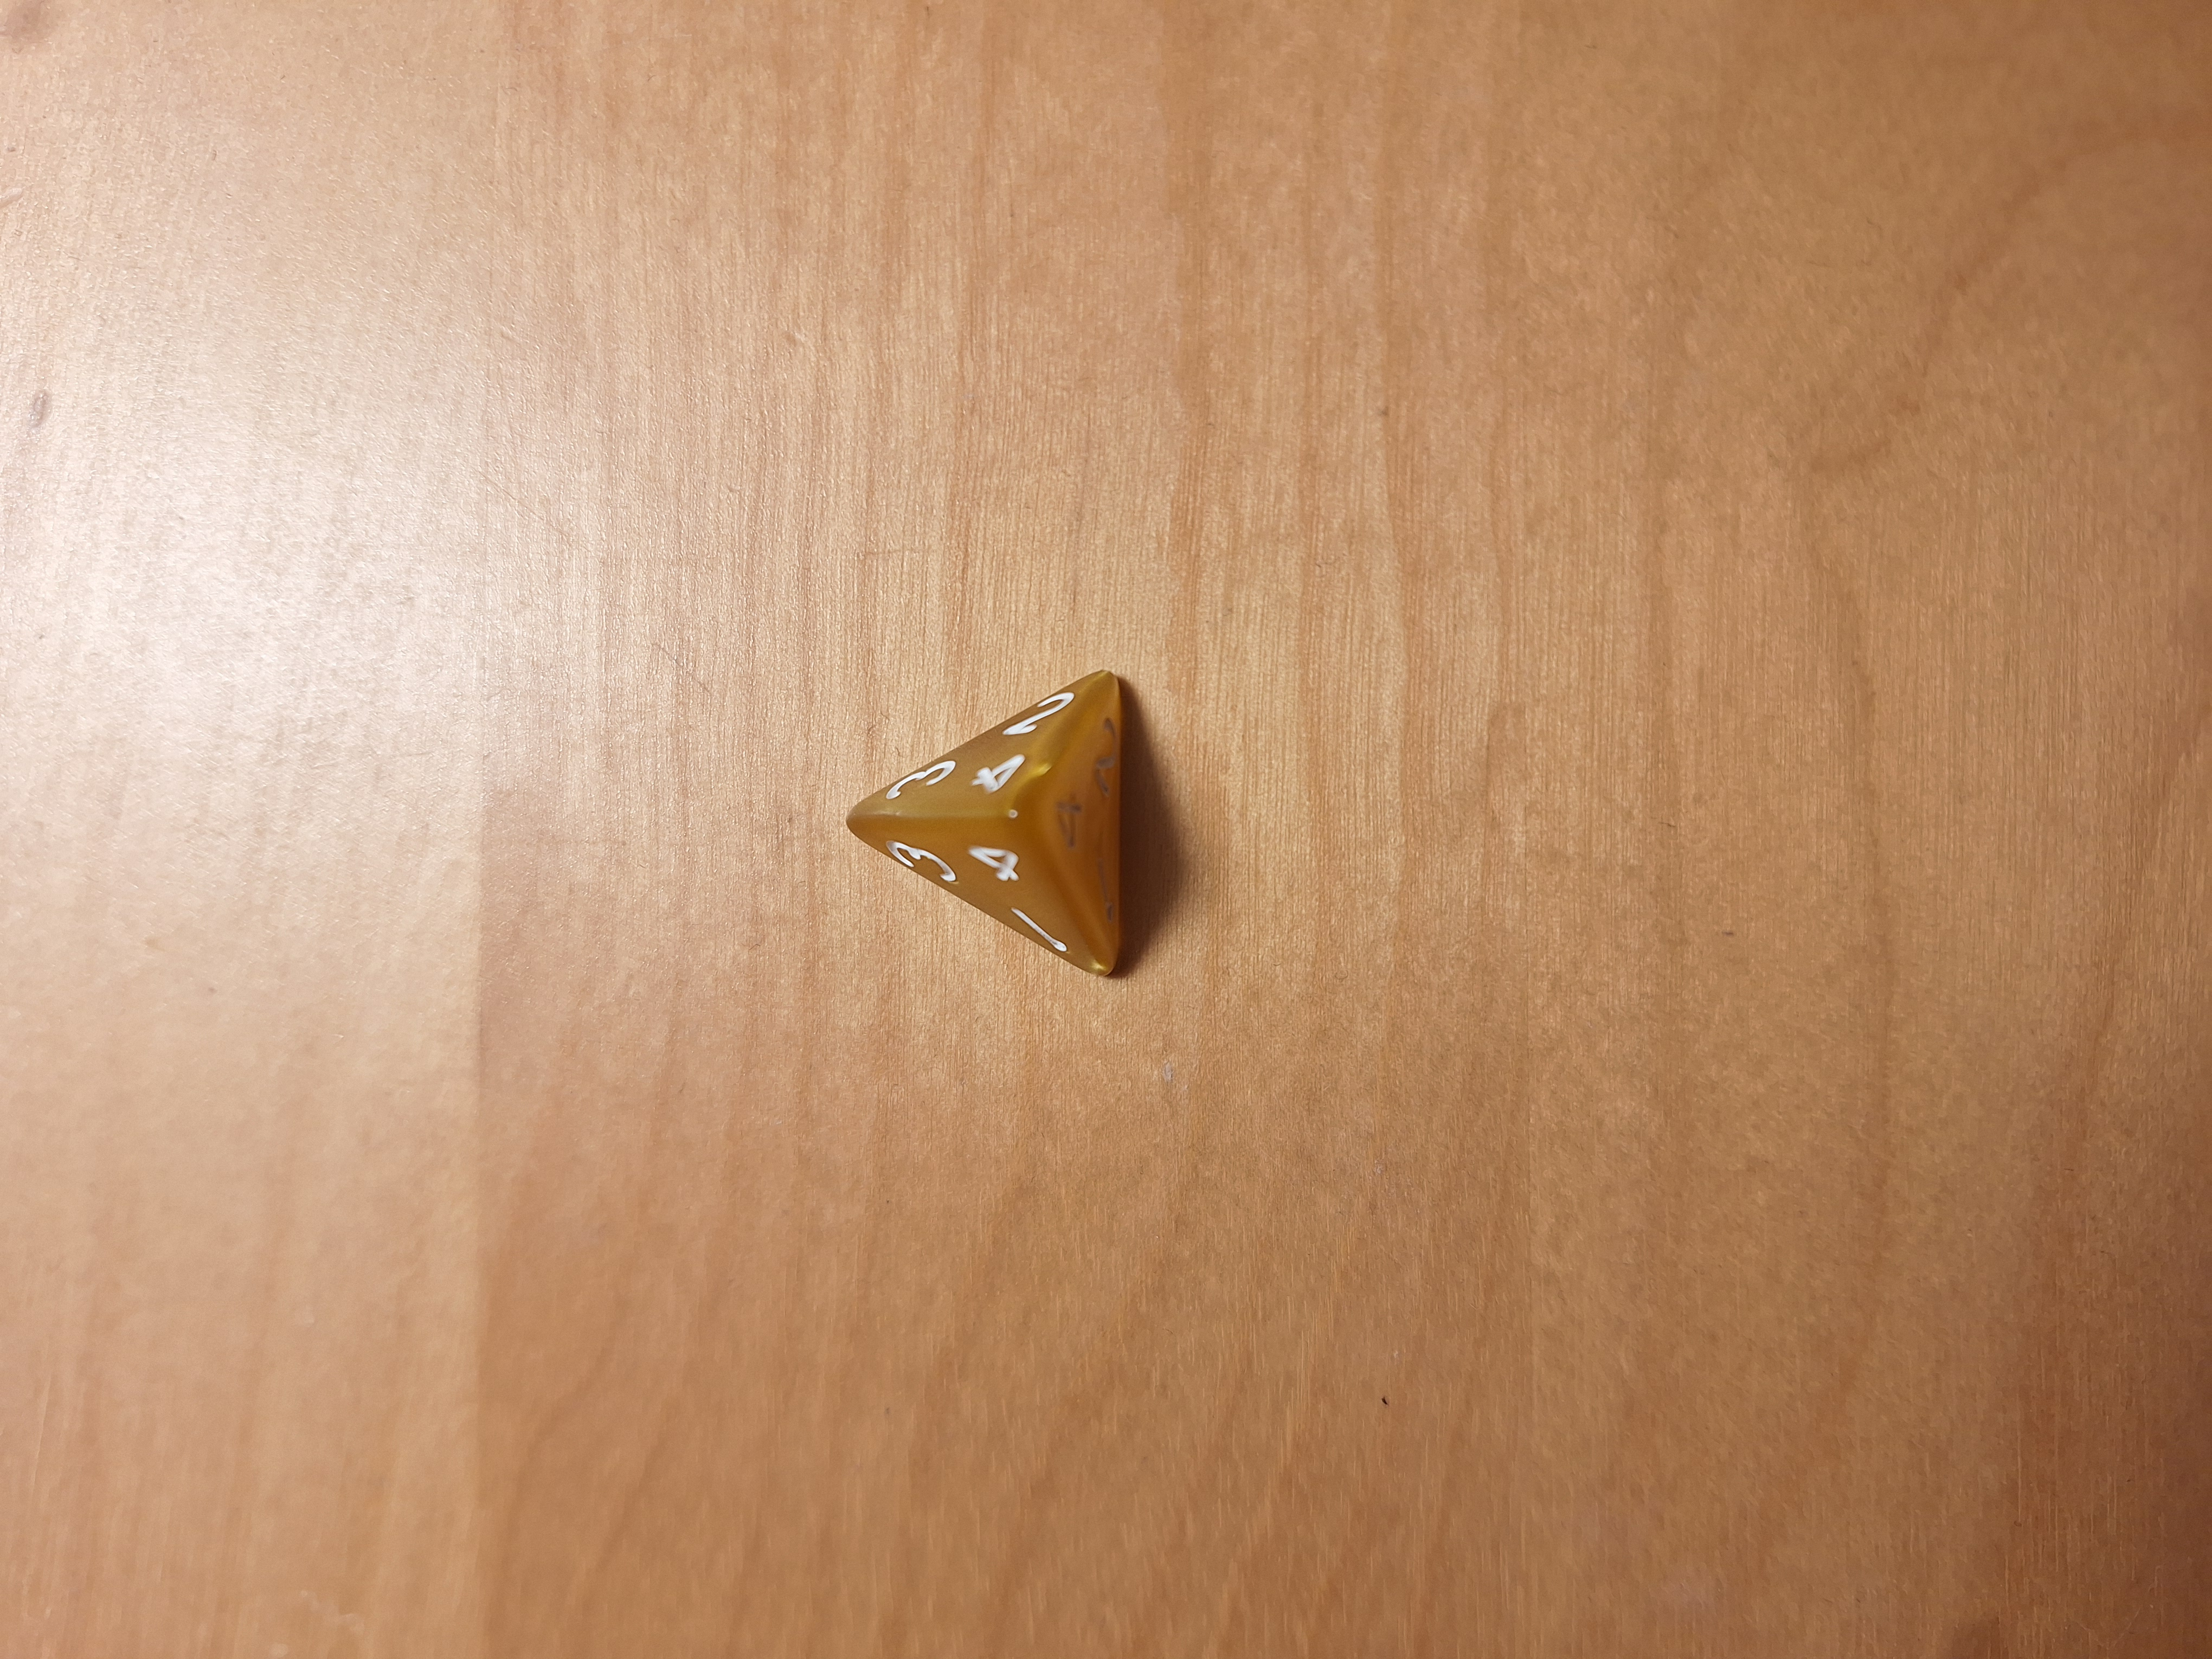
\includegraphics[width=.9\linewidth, angle=-90, clip]{chapters/02-teoria/figures/k4}
        \caption{\label{fig:k4}Kość czworościenna}
      \end{subfigure}%
      \begin{subfigure}{.3\textwidth}
        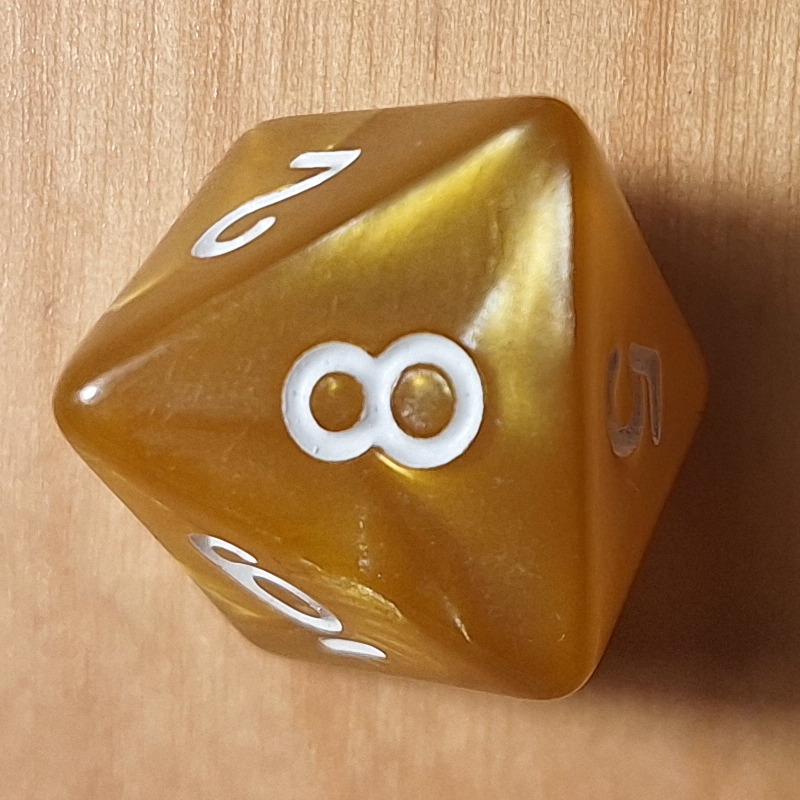
\includegraphics[width=.9\linewidth, angle=-90, clip]{chapters/02-teoria/figures/k8}
        \caption{\label{fig:k8}Kość ośmiościenna}
      \end{subfigure}%
       \begin{subfigure}{.3\textwidth}
        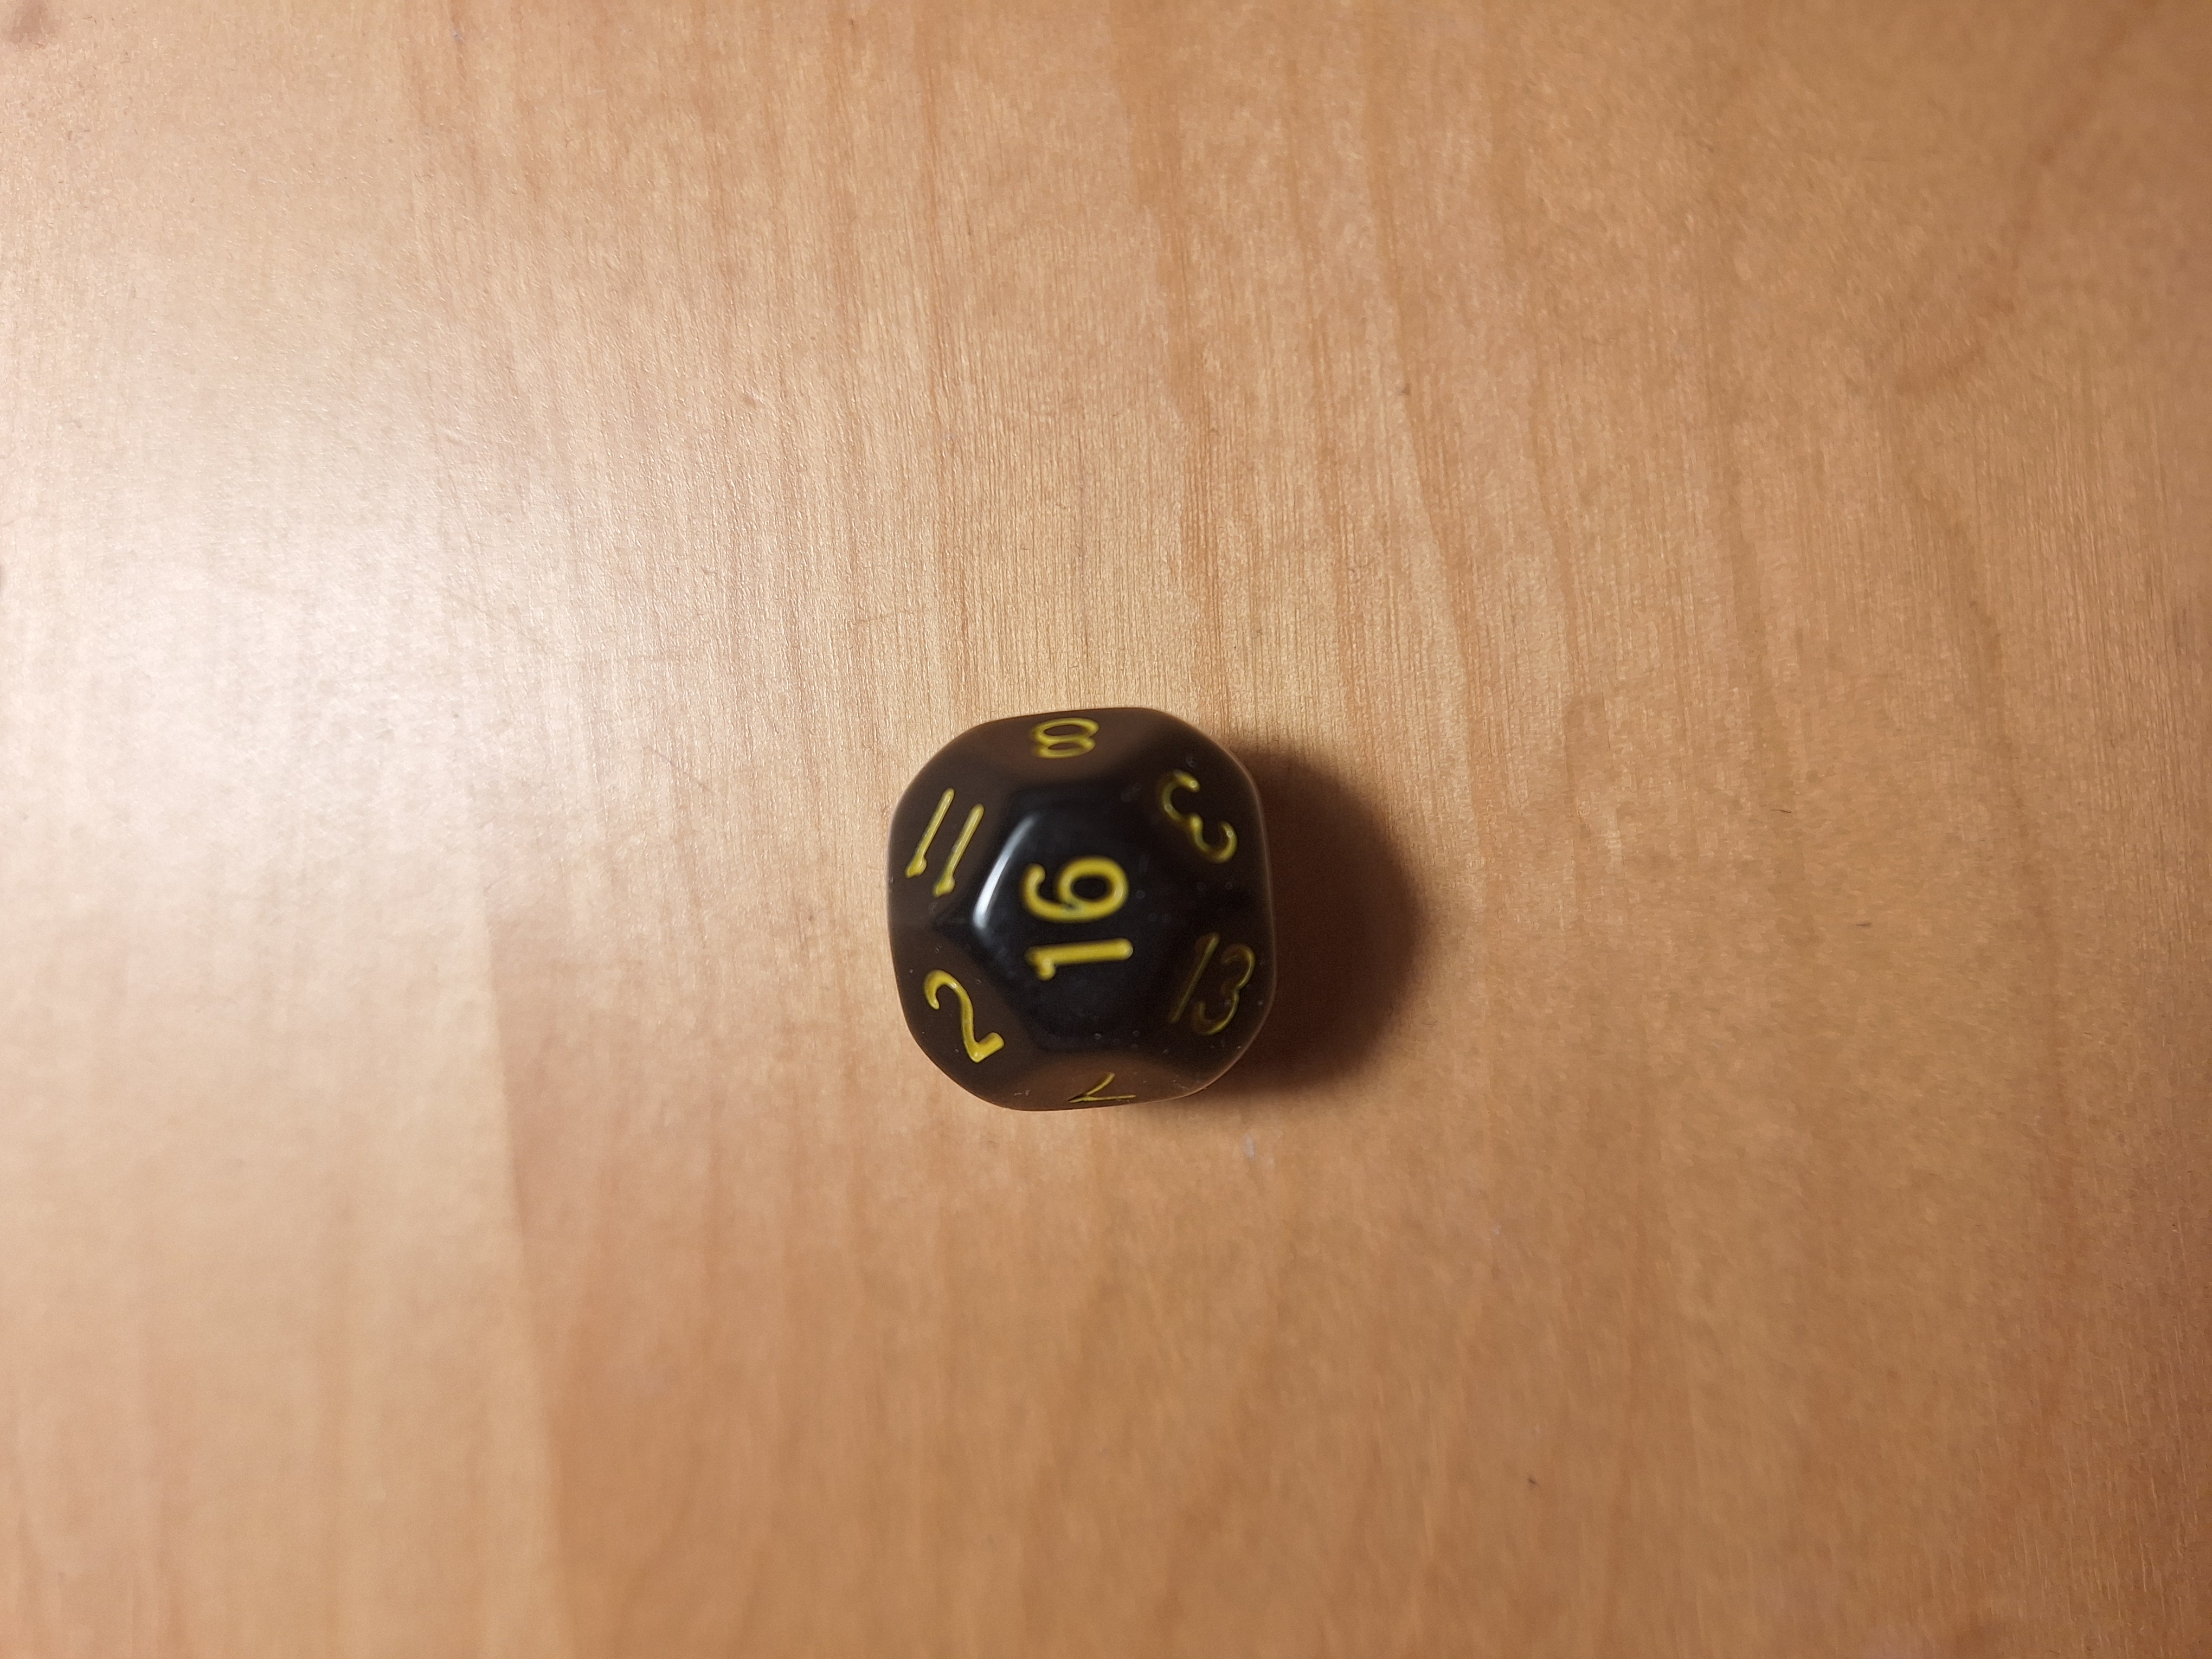
\includegraphics[width=.9\textwidth, angle=-90, clip]{chapters/02-teoria/figures/k16}
        \caption{\label{fig:k16}Kość szesnastościenna}
      \end{subfigure}
    \caption{Zdjęcia kości z góry}
\end{figure}

\begin{figure}[h]
    \centering
      \begin{subfigure}{.43\textwidth}
        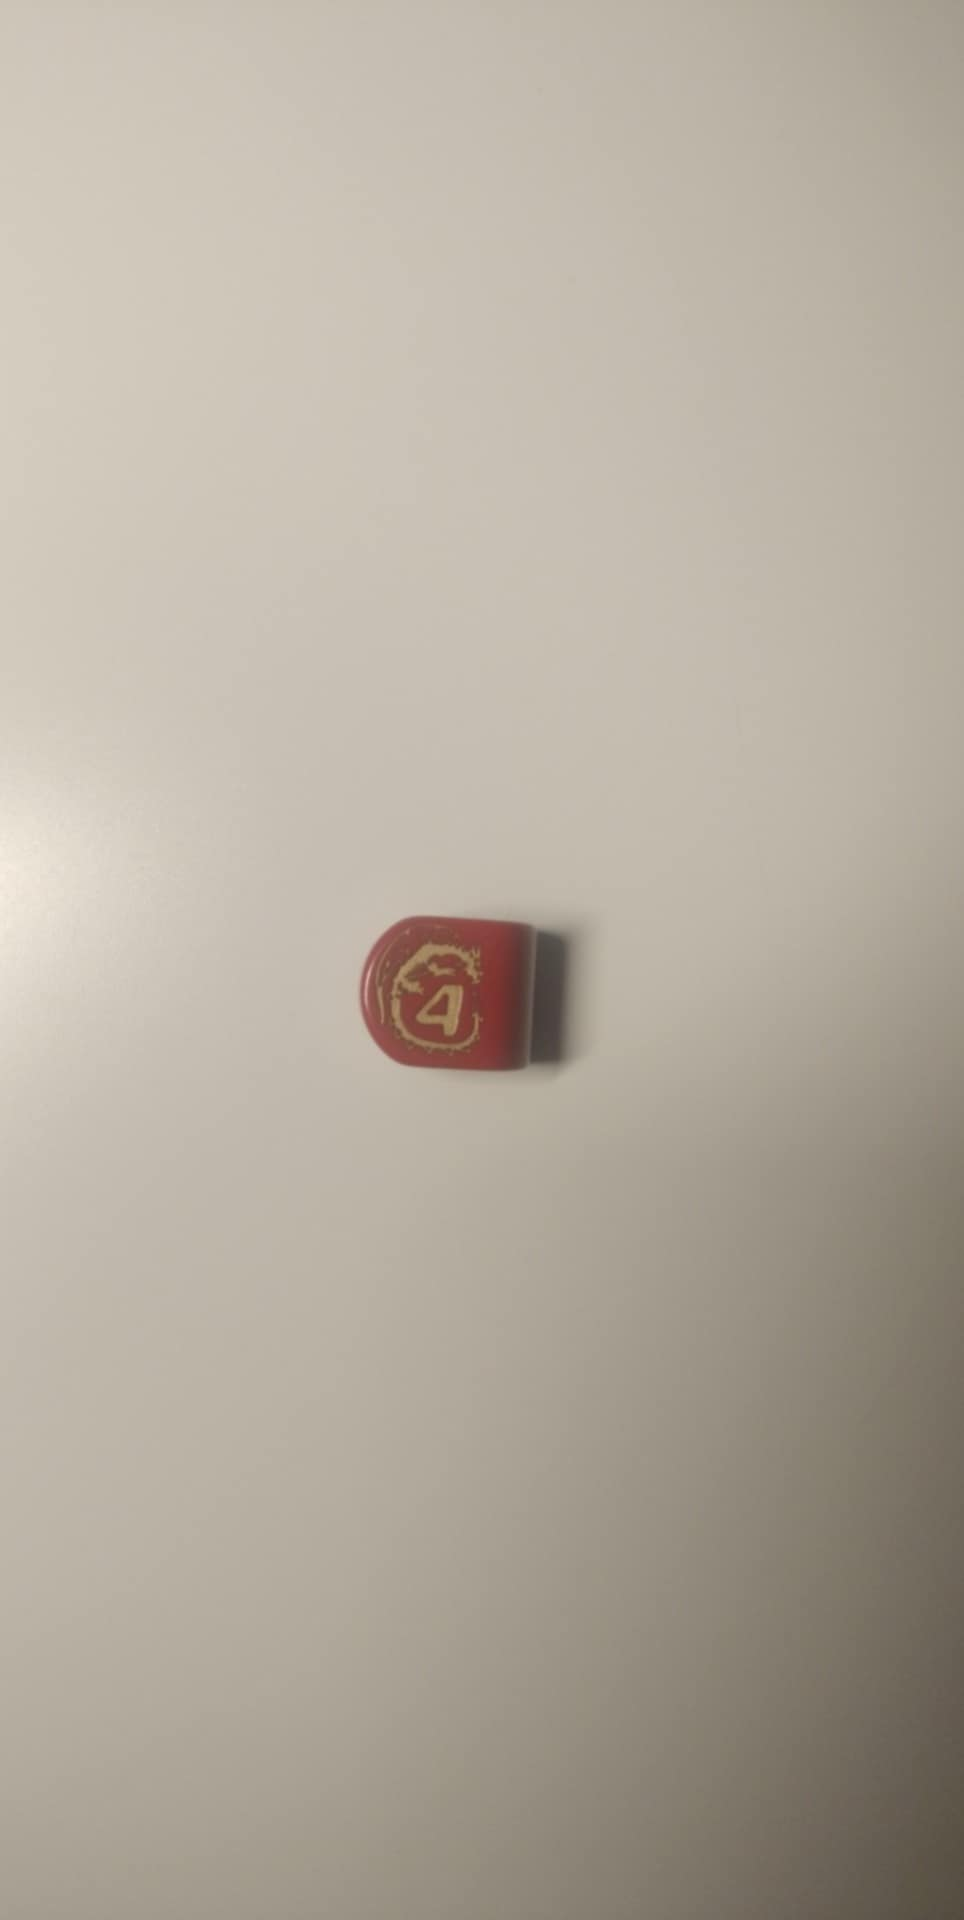
\includegraphics[width=.9\linewidth]{chapters/02-teoria/figures/modern_k4}
        \caption{\label{fig:modern_k4}Kość czworościenna typu „modern”}
      \end{subfigure}%
      \begin{subfigure}{.45\textwidth}
        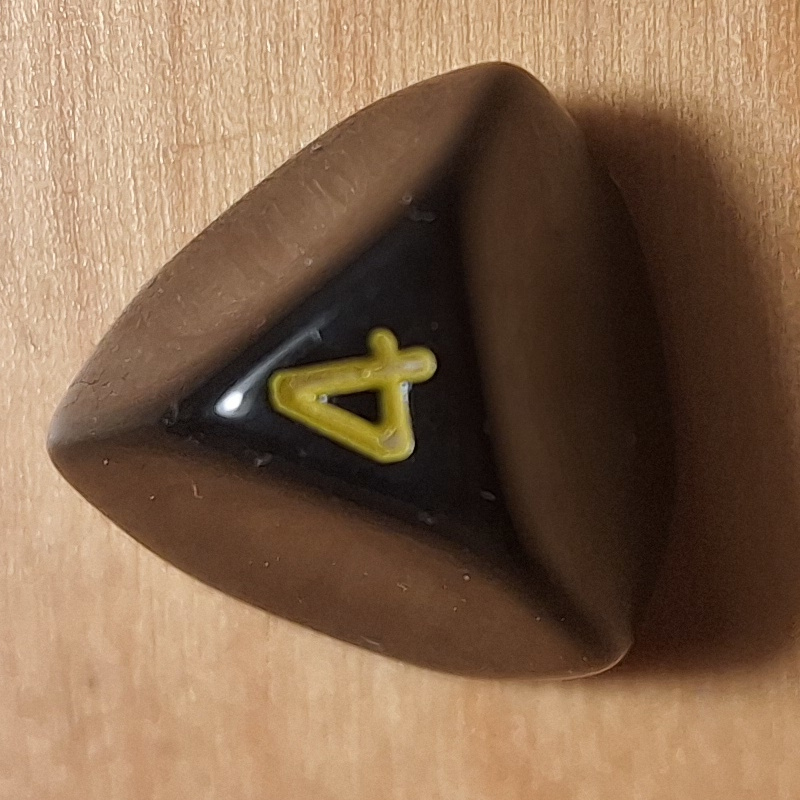
\includegraphics[width=.9\linewidth, angle=-90, clip]{chapters/02-teoria/figures/nietypowe_k4}
        \caption{\label{fig:nietypowe_k4}Kość czworościenna ze ściętym czubkiem}
      \end{subfigure}%
    \caption{Nietypowe kości czworościenne}
    \label{fig:nietypowe_modern_k4}
\end{figure}